\chapter{Návrh budoucí architektury kontejnerové aplikace}\label{sec:chap5}
V předchozích kapitolách byl představen koncept legacy aplikace a migrované aplikace. V této kapitole budou uvedeny směry, kterými lze řešení dále vyvíjet. Zároveň bude představen návrh a architektura nového řešení s důrazem kladeným na problémy zmíněné v kapitole číslo \ref{sec:chap4}. Migrovaná aplikace částečně používá zastaralou monolitickou architekturu. I přesto, že jsou služby logicky rozděleny na jednotlivé role a komponenty, je samotné řešení velmi složité na provoz a vývoj. Při škálování virtuálního control plane je nutné vytvářet nové virtuální stroje, které konzumují hardwarové zdroje, které nejsou efektivně využity.

\section{Současné možnosti}
V této části kapitoly budou představeny současné možnosti, pomocí kterých lze vybranou aplikaci (MCP) dále zlepšit a udržovat tak, aby byla stabilnější a jednodušší jak pro zákazníky, tak i pro servisní inženýry a vývojáře, kteří aplikaci vyvíjejí.
Prvním řešením je udržet a stabilizovat současné řešení, včetně životního cyklu aplikace. Obrovskou výhodou původního řešení je již zmiňovaná flexibilita, na kterou jsou zákazníci zvyklí a  již nemají u konkurenčních řešení. Prvním bodem pro stabilizaci současného řešení je nutnost standardizovat model, jak již bylo zmíněno v popisu instalace aplikace. Každé prostředí je postavené na vygenerovaném modelu, který je následně upravován inženýrem, jenž prostředí instaluje. A jelikož chybí systém osvědčených postupů, tak si každý inženýr upravuje model způsobem, aby byl pro něho přehledný. V praxi lze totiž namodelovat výslednou konfiguraci mnoha různými způsoby. Problémy odlišných modelů se následně stávají spornými během upgradu cloudu, kdy jednotlivé modely musí být opět upraveny, aby přidávaly nebo odebíraly jednotlivou funkcionalitu. V současnosti se tento problém řeší přesunem metadat z produktové (cluster) úrovně na systémovou, aby ubylo parametrů a produktová úroveň byla přehlednější. Model souvisí i s Jenkins pipelinami, pomocí kterých jsou jednotlivé akce vykonány. Koncept Jenkins pipeline byl popsán v kapitole \ref{sec:chap4}. Na tento problém bohužel neexistuje jedno univerzální řešení, které by bylo v případě Mirantisu potřeba.
Jak už bylo zmíněno v předchozí kapitole, OpenStack je globální projekt, který je vyvíjen mnoha vývojáři napříč firmami. Většinu těchto firem spojuje nejen zdrojový kód, který vývojáři píší, ale také vznikající problémy propojené s provozem a správou OpenStack cloudů. Z toho důvodu začalo nezávisle na sobě vznikat několik projektů, jak tyto problémy vyřešit. Kontejnerizace OpenStacku je zcela nový směr a způsob, jak provozovat OpenStack. S myšlenkou kontejnerizovaného OpenStacku začaly firmy experimentovat během prvních verzí k8s v roce 2015. Ani jedna firma v tu dobu nebyla schopna nabídnout žádný stabilní projekt či produkt. Z tohoto důvodu vzniklo hned několik projektů, které problém řeší. Pro ilustraci byly vybrány projekty s největší uživatelskou základnou:
\begin{itemize}
\item \textbf{Kolla} – První OpenStack projekt zabývající se sestavováním a nasazením OpenStacku do kontejnerového prostředí. K nasazování je použit konfigurační management Ansible \cite{kolla_ansible}. Dříve existoval projekt Kolla i pro Mesos a Kubernetes.
\item \textbf{OpenStack-Helm} – Další projekt spravovaný OpenStack Foundation, který se zabývá tvorbou a nasazením kontejnerů. Jak již název napovídá, jedná se o sadu Helm chartů, pomocí kterých lze OpenStack nainstalovat a spravovat.
\item \textbf{stackanetes} – Projekt, který vznikl ve spolupráci mezi firmami CoreOS a intel. Stackanetes se zabývá pouze instalací základních OpenStack službem, používá především nástroje vyvinuté firmou CoreOS, např. kpm. Po akvizici CoreOS Red Hatem byl tento projekt pozastaven a ve vývoji se již nepokračuje.
\item \textbf{AirShip} – Nejnovější řešení, které se stalo součástí OpenStack Foundation. Skládá se z kolekce několika projektů. Podle zdroje \cite{airship} jde spíše o framework, který řeší kompletní životní cyklus nejen OpenStacku, ale také operačního systému hostů a hardwaru. Celé AirShip řešení bylo vytvořeno firmami AT\&T, South Korea Telecom (SKT) a Intel, které pomocí něho chtějí provozovat svou infrastrukturu pro 5G.
\item \textbf{loci} – Projekt loci, na rozdíl od předchozích řešení, poskytuje pouze lehkotonážní Docker image, ovšem neřeší jejich nasazení a lifecycle management. Pomocí loci projektu lze jednoduše sestavovat image pro široké spektrum linuxových distrubcí s odlišnými balíčkovacími systémy (Debian, Censtos, Suse, atd.).
\end{itemize}

I přestože vývojáři Mirantisu přispívají do zmíněných projektů, v současné době žádný z projektů není zcela optimální pro nahrazení současného MCP. Hlavním cílem Mirantisu je mít nástroj, který vyřeší zmíněné problémy uvedené v kapitole \ref{sec:chap4} a ulehčí operátorům správu prostředí. Dále je nutné, aby kontejnerizované MCP bylo možné nasadit do jakéhokoliv k8s clusteru. To je důležité především kvůli uživatelské komunitě, která by si mohla řešení otestovat sama a podílet se na vývoji. S kontejnerizací přichází také řada nových problémů, které je nutno vyřešit. Prvním z nich je dodávání opravných záplat. V současné době jsou opravy dodávány debian balíčky. Balíčky jsou uloženy v repozitáři, který je unikátní pro každou verzi. Odlišení verzí je implementováno pomocí tagu. Tag je vždy unikátní pro danou verzi. V případě Mirantisu jsou vydané verze označeny rokem, měsícem a opravnou revizí, kdy byla verze vydána (např. 2018.4.1). Při použití kontejnerizace verzování balíčků už není potřeba, jelikož všechny komponenty budou spouštěny v rámci kontejnerů. Bezpečnostní záplaty budou fungovat následovně. Objeví-li se chyba v produktu, bude opraven zdrojový kód a sestaví se nový Docker image se stejným tagem, jaký byl použit pro vybranou verzi. Zákazník poté nebude muset stále kontrolovat, zda má nainstalované nejnovější balíčky a jejich závislosti. Veškeré aktualizace budou prováděny pomocí nasazení nových kontejnerů, které budou nasazeny formou rolling aktualizace, což znamená, že jednotlivé záplaty bude možno aplikovat bezvýpadkově. Největší problém se týká migrace stávajících zákazníků. Jedná se především o migraci workloadu ovládaného OpenStackem. Tento typ migrace je technicky velmi složitý. Aby migrace byla co nejméně bezvýpadková, je nutno vytvořit vedle současného clusteru také cluster kontejnerový, kde bude nové řešení naimplementováno. Postupně k němu budou připojeny compute servery s migrovaným workloadem. Velmi důležité je umístění disků jednotlivých instancí. Jsou-li disky uloženy v externí storage mimo cloud, tak migrace nebude obtížná. V tomto případě stačí pouze přesunout databázi, kterou lze převést pomocí obnovení záloh, které jsou periodicky vytvářeny. V databázi jsou uvedeny jednotlivé cesty na disky ve storage. Stačí připojit storage ke kontejnerovému řešení a instance znovu spustit. Pro disky ukládané přímo na souborový systém compute serveru bude tento proces časově i technicky náročnější. Proto se zvažuje několik možných řešení, jak s těmito prostředími nakládat. Tím nejpravděpodobnějším je nemigrovat a udržovat prostředí pomocí současných nástrojů. Zákazníkům budou dodávány pouze bezpečnostní záplaty. Nové vlastnosti budou dostupné až v rámci kontejnerového řešení, upgrade na kontejnerové řešení by se řešil přeinstalací celého prostředí.

\section{Definice požadavků}
V předchozí části kapitoly byla představena současná řešení, která ukazují jak představenou aplikaci MCP spravovat a vyvíjet dál. Pro jednodušší provoz OpenStacku nakonec byla zvolena možnost migrace do kontejnerového řešení. Orchestrátor je schopen zajistit spoustu úloh, které se musely řešit v předchozí architektuře externími nástroji, například vysoká dostupnost. Budoucí platforma musí být navržena tak, aby splňovala všechny funkční požadavky,které jsou od nového řešení očekávány.
\begin{itemize}
\item Prvním požadavkem je komplexnost. Podporuje stejné množství vlastností jako předchozí řešení a je velmi snadno konfigurovatelné. To platí o rozšiřitelnosti řešení, která by měla podporovat stejné spektrum integrací jako současné řešení postavené na virtuálních strojích.
\item Dalším aspektem je nasazování nového řešení. Řešení by nemělo být závislé pouze na jedné instalační metodě a mělo by podporovat více operačních systémů. Pro tento případ je výhodné používat k8s, který může být spuštěn nad jakoukoliv Linuxovou distribucí. Kontejnery jsou pak závislé jenom na zdrojích jádra. To znamená, že aplikace, která běží v kontejnerech, je závislá pouze na knihovnách, které jsou součástí kontejneru. Dále se otevírá možnost pro instalace řešení do k8s clusterů třetích stran, které nejsou spravovány Mirantisem, jelikož OpenStack control plane se může brát jako klasická kontejnerová aplikace.
\item Nejdůležitějším požadavkem pro nové řešení je mít systém, pomocí kterého lze jednoduše ovládat životní cyklus aplikace. Aplikaci by mělo jít jednoduše spravovat z jednoho místa a veškeré akce by měly být automatizované tak, že abstrahují operátory aplikace od komplexnosti.
\item Dalším požadavkem je mít spuštěno pouze tolik replik OpenStack služeb, které jsou v daný moment potřeba. Efektivně utilizovat hardwarové zdroje bez nutnosti spuštění replikovaných služeb. Díky k8s lze provádět rovněž dynamické škálování jednotlivých služeb. Pokud budou jednotlivé služby vytížené, automaticky se spustí další repliky.
\item Řešení by mělo být modulární, aby do něho bylo možné jednoduše přidávat další projekty a integrace na další služby. Výhodou modulárních řešení z pohledu OpenStacku je kombinace několika odlišných verzí komponent mezi sebou. Často se stává, i když to není v dokumentaci doporučováno, že je spuštěno několik OpenStack komponent se staršími verzemi. Jedná se většinou o komponenty Cinderu, která zajišťuje block storage. Zákazníci totiž chtějí používat jejich storage systémy, které mají kompatibilní ovladače pouze se zastaralými verzemi Cinderu. V tomto případě je tedy nutné Cinder spouštět ve starší verzi.
\item Poslední požadavek se týká testování. Díky odlehčenému modelu by pro testovací prostředí měly stačit mnohem menší clustery, které nezabírají tolik zdrojů a jejich spuštění trvá méně času.
\end{itemize}

\section{Návrh budoucí architektury kontejnerové aplikace}
Architektura systému je zobrazena na obrázku \ref{fig:openstack_operator}. Nová architektura bude postavena nad orchestrátorem k8s, jenž bude využíván pro orchestraci workloadu konceptu operátoru. Operátor se bude starat jak o nasazení aplikace, tak o její životní cyklus. Jednotlivé OpenStack komponenty budou rozděleny do kontejnerů. Jeden kontejner bude obsahovat vždy jednu službu komponenty. Například nova služba bude mít kontejnery pro služby nova-api, nova-scheduler, nova-conductor, nova-compute atd. Tyto kontejnery je nutné rozdělit do logických skupin (podů), v rámci kterých budou kontejnery spouštěny a škálovány. Protože podle zdroje \cite{k8s_devs} není vhodné mít všechny kontejnery od jedné služby v jednom podu. Při vytížení jednotlivých komponent, např. zmíněné novy, je nutné převážně škálovat api \cite{nova_scale}, nikoliv celou komponentu. Proto v rámci operátoru bude každá OpenStack komponenta mít svůj vlastní controller, který bude sloužit k provozu a hlídání nadefinovaných akcí. Tento controller rozšiřuje možnosti k8s reagovat na vytvořené CR (Custom Resource). CR je k8s objekt, je stejný jako k8s předdefinované objekty (např. pod, services, deployment, atd). Pokud je vytvořen požadavek s tímto typem objektu, k8s zkontroluje, zda existuje CRD předpis, který udává, zda daný cluster takový typ objektu zná. Pokud ano, je tento objekt poslán na operátor, který už podle zadaných parametrů dokáže provést manifestem stanovené akce. Zároveň lze pomocí controllerů sledovat jednotlivé stavy objektů a reagovat na ně. Při instalaci lze například ověřit, zda některé objekty existují, nebo zda je nutné počkat, než se vytvoří. Výhodou použití operátoru je především flexibilita přístupu. Samotný operátor je aplikací, jejíž logiku lze naprogramovat. Z obrázku se schématem je patrné, jak jednotlivé CR objekty spravují kontejnery s jednotlivými službami. Služby jsou mezi sebou propojeny pomocí cluster IP v rámci k8s služby. OpenStack je pro koncové uživatele dostupný přes Keystone public endpointy, které jsou vystavené na k8s službě jako externí ip adresa. Tato externí adresa je implementována formou k8s load balanceru. S těmito endpointy už může koncový uživatel pracovat stejně jako u klasického OpenStacku. Služby jsou pro přístup dostupné pomocí keystonerc souboru a OpenStack CLI klienta nebo přes grafické rozhraní Horizon.

\begin{figure}[H]
\begin{centering}
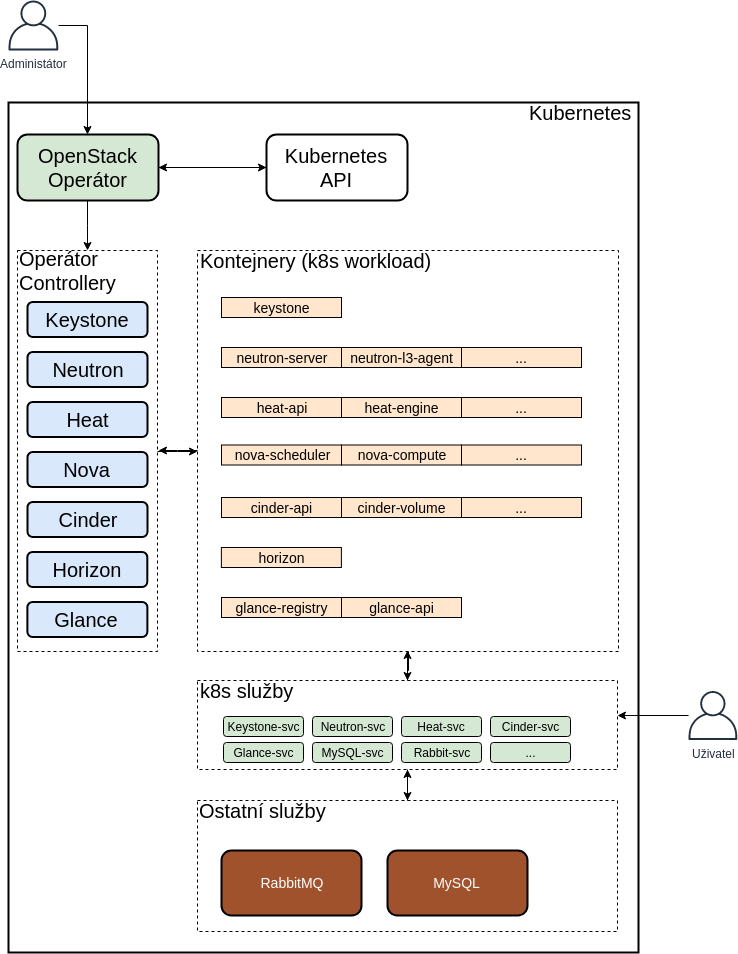
\includegraphics[width=0.9\textwidth]{img/openstack_operator.png}
\par\end{centering}
\caption{Návrh kontejnerové architektury, zdroj: vlastní tvorba} \label{fig:openstack_operator}
\end{figure}

Jak již bylo zmíněno v požadavcích, navrhované řešení je koncipováno, aby ho bylo možné nainstalovat do jakéhokoliv k8s clusteru. Nezáleží na nástroji, jakým byl cluster nainstalován. Je nutno zmínit, že vybraný k8s cluster, do něhož bude OpenStack nainstalován, musí mít připojený nějaký typ storage. Pro některé komponenty, např. MySQL databáze či Keystone, je nutné uchovávat perzistentní data mimo kontejner. Instalace samotného OpenStacku je velmi jednoduchá. Celá aplikace bude instalována a řízena pomocí OpenStack operátoru. Tento operátor lze nainstalovat dvěma způsoby. Prvním způsob je instalace pomocí manifestu, tedy nejprve bude do k8s aplikován předpis, který spustí kontejner s operátorem. Ten vytvoří sadu CRD, a bude tak možno použít manifesty s CR, které jsou již specializované pro OpenStack. Před aplikací jednotlivých CR je nutné spustit podpůrné služby, jako jsou MySQL databáze a RabbitMQ, které jsou OpenStackem vyžadovány. Tyto dvě aplikace opět mohou být instalovány několika způsoby. Jelikož se jedná o aplikace, které mohou být provozovány nezávisle, nebyly proto přidány do OpenStack operátoru. Pro obě aplikace existují vlastní operátory. Po spuštění a konfiguraci těchto dvou aplikací lze popořadě aplikovat manifesty s CR, které spustí postupně control plane. Druhým způsobem je použití helm chartu pro OpenStack operátor, který má jednotlivé manifesty pro CRD a CR uložené v šablonách.
